\documentclass[1p]{elsarticle_modified}
%\bibliographystyle{elsarticle-num}

%\usepackage[colorlinks]{hyperref}
%\usepackage{abbrmath_seonhwa} %\Abb, \Ascr, \Acal ,\Abf, \Afrak
\usepackage{amsfonts}
\usepackage{amssymb}
\usepackage{amsmath}
\usepackage{amsthm}
\usepackage{scalefnt}
\usepackage{amsbsy}
\usepackage{kotex}
\usepackage{caption}
\usepackage{subfig}
\usepackage{color}
\usepackage{graphicx}
\usepackage{xcolor} %% white, black, red, green, blue, cyan, magenta, yellow
\usepackage{float}
\usepackage{setspace}
\usepackage{hyperref}

\usepackage{tikz}
\usetikzlibrary{arrows}

\usepackage{multirow}
\usepackage{array} % fixed length table
\usepackage{hhline}

%%%%%%%%%%%%%%%%%%%%%
\makeatletter
\renewcommand*\env@matrix[1][\arraystretch]{%
	\edef\arraystretch{#1}%
	\hskip -\arraycolsep
	\let\@ifnextchar\new@ifnextchar
	\array{*\c@MaxMatrixCols c}}
\makeatother %https://tex.stackexchange.com/questions/14071/how-can-i-increase-the-line-spacing-in-a-matrix
%%%%%%%%%%%%%%%

\usepackage[normalem]{ulem}

\newcommand{\msout}[1]{\ifmmode\text{\sout{\ensuremath{#1}}}\else\sout{#1}\fi}
%SOURCE: \msout is \stkout macro in https://tex.stackexchange.com/questions/20609/strikeout-in-math-mode

\newcommand{\cancel}[1]{
	\ifmmode
	{\color{red}\msout{#1}}
	\else
	{\color{red}\sout{#1}}
	\fi
}

\newcommand{\add}[1]{
	{\color{blue}\uwave{#1}}
}

\newcommand{\replace}[2]{
	\ifmmode
	{\color{red}\msout{#1}}{\color{blue}\uwave{#2}}
	\else
	{\color{red}\sout{#1}}{\color{blue}\uwave{#2}}
	\fi
}

\newcommand{\Sol}{\mathcal{S}} %segment
\newcommand{\D}{D} %diagram
\newcommand{\A}{\mathcal{A}} %arc


%%%%%%%%%%%%%%%%%%%%%%%%%%%%%5 test

\def\sl{\operatorname{\textup{SL}}(2,\Cbb)}
\def\psl{\operatorname{\textup{PSL}}(2,\Cbb)}
\def\quan{\mkern 1mu \triangleright \mkern 1mu}

\theoremstyle{definition}
\newtheorem{thm}{Theorem}[section]
\newtheorem{prop}[thm]{Proposition}
\newtheorem{lem}[thm]{Lemma}
\newtheorem{ques}[thm]{Question}
\newtheorem{cor}[thm]{Corollary}
\newtheorem{defn}[thm]{Definition}
\newtheorem{exam}[thm]{Example}
\newtheorem{rmk}[thm]{Remark}
\newtheorem{alg}[thm]{Algorithm}

\newcommand{\I}{\sqrt{-1}}
\begin{document}

%\begin{frontmatter}
%
%\title{Boundary parabolic representations of knots up to 8 crossings}
%
%%% Group authors per affiliation:
%\author{Yunhi Cho} 
%\address{Department of Mathematics, University of Seoul, Seoul, Korea}
%\ead{yhcho@uos.ac.kr}
%
%
%\author{Seonhwa Kim} %\fnref{s_kim}}
%\address{Center for Geometry and Physics, Institute for Basic Science, Pohang, 37673, Korea}
%\ead{ryeona17@ibs.re.kr}
%
%\author{Hyuk Kim}
%\address{Department of Mathematical Sciences, Seoul National University, Seoul 08826, Korea}
%\ead{hyukkim@snu.ac.kr}
%
%\author{Seokbeom Yoon}
%\address{Department of Mathematical Sciences, Seoul National University, Seoul, 08826,  Korea}
%\ead{sbyoon15@snu.ac.kr}
%
%\begin{abstract}
%We find all boundary parabolic representation of knots up to 8 crossings.
%
%\end{abstract}
%\begin{keyword}
%    \MSC[2010] 57M25 
%\end{keyword}
%
%\end{frontmatter}

%\linenumbers
%\tableofcontents
%
\newcommand\colored[1]{\textcolor{white}{\rule[-0.35ex]{0.8em}{1.4ex}}\kern-0.8em\color{red} #1}%
%\newcommand\colored[1]{\textcolor{white}{ #1}\kern-2.17ex	\textcolor{white}{ #1}\kern-1.81ex	\textcolor{white}{ #1}\kern-2.15ex\color{red}#1	}

{\Large $\underline{11a_{259}~(K11a_{259})}$}

\setlength{\tabcolsep}{10pt}
\renewcommand{\arraystretch}{1.6}
\vspace{1cm}\begin{tabular}{m{100pt}>{\centering\arraybackslash}m{274pt}}
\multirow{5}{120pt}{
	\centering
	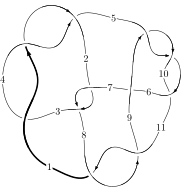
\includegraphics[width=112pt]{../../../GIT/diagram.site/Diagrams/png/508_11a_259.png}\\
\ \ \ A knot diagram\footnotemark}&
\allowdisplaybreaks
\textbf{Linearized knot diagam} \\
\cline{2-2}
 &
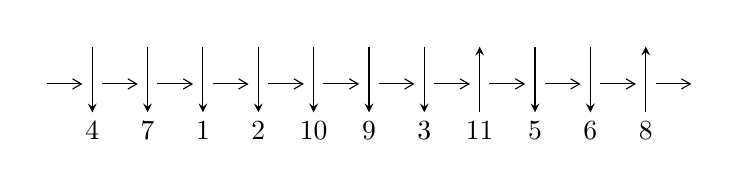
\begin{tikzpicture}[x=20pt, y=17pt]
	% nodes
	\node (C0) at (0, 0) {};
	\node (C1) at (1, 0) {};
	\node (C1U) at (1, +1) {};
	\node (C1D) at (1, -1) {4};

	\node (C2) at (2, 0) {};
	\node (C2U) at (2, +1) {};
	\node (C2D) at (2, -1) {7};

	\node (C3) at (3, 0) {};
	\node (C3U) at (3, +1) {};
	\node (C3D) at (3, -1) {1};

	\node (C4) at (4, 0) {};
	\node (C4U) at (4, +1) {};
	\node (C4D) at (4, -1) {2};

	\node (C5) at (5, 0) {};
	\node (C5U) at (5, +1) {};
	\node (C5D) at (5, -1) {10};

	\node (C6) at (6, 0) {};
	\node (C6U) at (6, +1) {};
	\node (C6D) at (6, -1) {9};

	\node (C7) at (7, 0) {};
	\node (C7U) at (7, +1) {};
	\node (C7D) at (7, -1) {3};

	\node (C8) at (8, 0) {};
	\node (C8U) at (8, +1) {};
	\node (C8D) at (8, -1) {11};

	\node (C9) at (9, 0) {};
	\node (C9U) at (9, +1) {};
	\node (C9D) at (9, -1) {5};

	\node (C10) at (10, 0) {};
	\node (C10U) at (10, +1) {};
	\node (C10D) at (10, -1) {6};

	\node (C11) at (11, 0) {};
	\node (C11U) at (11, +1) {};
	\node (C11D) at (11, -1) {8};
	\node (C12) at (12, 0) {};

	% arrows
	\draw[->,>={angle 60}]
	(C0) edge (C1) (C1) edge (C2) (C2) edge (C3) (C3) edge (C4) (C4) edge (C5) (C5) edge (C6) (C6) edge (C7) (C7) edge (C8) (C8) edge (C9) (C9) edge (C10) (C10) edge (C11) (C11) edge (C12) ;	\draw[->,>=stealth]
	(C1U) edge (C1D) (C2U) edge (C2D) (C3U) edge (C3D) (C4U) edge (C4D) (C5U) edge (C5D) (C6U) edge (C6D) (C7U) edge (C7D) (C8D) edge (C8U) (C9U) edge (C9D) (C10U) edge (C10D) (C11D) edge (C11U) ;
	\end{tikzpicture} \\
\hhline{~~} \\& 
\textbf{Solving Sequence} \\ \cline{2-2} 
 &
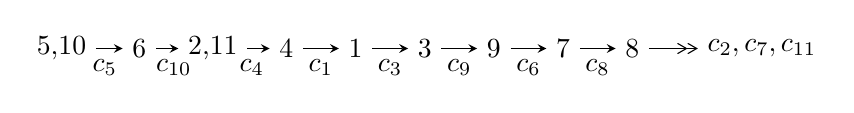
\begin{tikzpicture}[x=25pt, y=7pt]
	% node
	\node (A0) at (-1/8, 0) {5,10};
	\node (A1) at (1, 0) {6};
	\node (A2) at (33/16, 0) {2,11};
	\node (A3) at (25/8, 0) {4};
	\node (A4) at (33/8, 0) {1};
	\node (A5) at (41/8, 0) {3};
	\node (A6) at (49/8, 0) {9};
	\node (A7) at (57/8, 0) {7};
	\node (A8) at (65/8, 0) {8};
	\node (C1) at (1/2, -1) {$c_{5}$};
	\node (C2) at (3/2, -1) {$c_{10}$};
	\node (C3) at (21/8, -1) {$c_{4}$};
	\node (C4) at (29/8, -1) {$c_{1}$};
	\node (C5) at (37/8, -1) {$c_{3}$};
	\node (C6) at (45/8, -1) {$c_{9}$};
	\node (C7) at (53/8, -1) {$c_{6}$};
	\node (C8) at (61/8, -1) {$c_{8}$};
	\node (A9) at (10, 0) {$c_{2},c_{7},c_{11}$};

	% edge
	\draw[->,>=stealth]	
	(A0) edge (A1) (A1) edge (A2) (A2) edge (A3) (A3) edge (A4) (A4) edge (A5) (A5) edge (A6) (A6) edge (A7) (A7) edge (A8) ;
	\draw[->>,>={angle 60}]	
	(A8) edge (A9);
\end{tikzpicture} \\ 

\end{tabular} \\

\footnotetext{
The image of knot diagram is generated by the software ``\textbf{Draw programme}" developed by Andrew Bartholomew(\url{http://www.layer8.co.uk/maths/draw/index.htm\#Running-draw}), where we modified some parts for our purpose(\url{https://github.com/CATsTAILs/LinksPainter}).
}\phantom \\ \newline 
\centering \textbf{Ideals for irreducible components\footnotemark of $X_{\text{par}}$} 
 
\begin{align*}
I^u_{1}&=\langle 
u^{43}+u^{42}+\cdots+b- u,\;u^{43}+u^{42}+\cdots+a-2,\;u^{44}+2 u^{43}+\cdots-3 u-1\rangle \\
I^u_{2}&=\langle 
b+1,\;u^3+a-2 u+1,\;u^5+u^4-2 u^3- u^2+u-1\rangle \\
\\
\end{align*}
\raggedright * 2 irreducible components of $\dim_{\mathbb{C}}=0$, with total 49 representations.\\
\footnotetext{All coefficients of polynomials are rational numbers. But the coefficients are sometimes approximated in decimal forms when there is not enough margin.}
\newpage
\renewcommand{\arraystretch}{1}
\centering \section*{I. $I^u_{1}= \langle u^{43}+u^{42}+\cdots+b- u,\;u^{43}+u^{42}+\cdots+a-2,\;u^{44}+2 u^{43}+\cdots-3 u-1 \rangle$}
\flushleft \textbf{(i) Arc colorings}\\
\begin{tabular}{m{7pt} m{180pt} m{7pt} m{180pt} }
\flushright $a_{5}=$&$\begin{pmatrix}1\\0\end{pmatrix}$ \\
\flushright $a_{10}=$&$\begin{pmatrix}0\\u\end{pmatrix}$ \\
\flushright $a_{6}=$&$\begin{pmatrix}1\\u^2\end{pmatrix}$ \\
\flushright $a_{2}=$&$\begin{pmatrix}- u^{43}- u^{42}+\cdots+6 u+2\\- u^{43}- u^{42}+\cdots+3 u^2+u\end{pmatrix}$ \\
\flushright $a_{11}=$&$\begin{pmatrix}- u\\- u^3+u\end{pmatrix}$ \\
\flushright $a_{4}=$&$\begin{pmatrix}-2 u^{43}-2 u^{42}+\cdots+7 u+3\\- u^{43}- u^{42}+\cdots+11 u^3+2 u^2\end{pmatrix}$ \\
\flushright $a_{1}=$&$\begin{pmatrix}- u^9+4 u^7-5 u^5+2 u^3- u\\- u^{11}+5 u^9-8 u^7+3 u^5+u^3+u\end{pmatrix}$ \\
\flushright $a_{3}=$&$\begin{pmatrix}-3 u^{43}-3 u^{42}+\cdots+6 u+3\\- u^{43}- u^{42}+\cdots-17 u^4+6 u^3\end{pmatrix}$ \\
\flushright $a_{9}=$&$\begin{pmatrix}u\\u\end{pmatrix}$ \\
\flushright $a_{7}=$&$\begin{pmatrix}- u^4+u^2+1\\- u^4+2 u^2\end{pmatrix}$ \\
\flushright $a_{8}=$&$\begin{pmatrix}u^5-2 u^3+u\\u^7-3 u^5+2 u^3+u\end{pmatrix}$\\ \flushright $a_{8}=$&$\begin{pmatrix}u^5-2 u^3+u\\u^7-3 u^5+2 u^3+u\end{pmatrix}$\\&\end{tabular}
\flushleft \textbf{(ii) Obstruction class $= -1$}\\~\\
\flushleft \textbf{(iii) Cusp Shapes $= 2 u^{43}+4 u^{42}+\cdots+u-10$}\\~\\
\newpage\renewcommand{\arraystretch}{1}
\flushleft \textbf{(iv) u-Polynomials at the component}\newline \\
\begin{tabular}{m{50pt}|m{274pt}}
Crossings & \hspace{64pt}u-Polynomials at each crossing \\
\hline $$\begin{aligned}c_{1},c_{3},c_{4}\end{aligned}$$&$\begin{aligned}
&u^{44}-6 u^{43}+\cdots+3 u-1
\end{aligned}$\\
\hline $$\begin{aligned}c_{2},c_{7}\end{aligned}$$&$\begin{aligned}
&u^{44}- u^{43}+\cdots+32 u+32
\end{aligned}$\\
\hline $$\begin{aligned}c_{5},c_{9},c_{10}\end{aligned}$$&$\begin{aligned}
&u^{44}+2 u^{43}+\cdots-3 u-1
\end{aligned}$\\
\hline $$\begin{aligned}c_{6}\end{aligned}$$&$\begin{aligned}
&u^{44}-6 u^{43}+\cdots+175 u+53
\end{aligned}$\\
\hline $$\begin{aligned}c_{8},c_{11}\end{aligned}$$&$\begin{aligned}
&u^{44}+6 u^{43}+\cdots-57 u-9
\end{aligned}$\\
\hline
\end{tabular}\\~\\
\newpage\renewcommand{\arraystretch}{1}
\flushleft \textbf{(v) Riley Polynomials at the component}\newline \\
\begin{tabular}{m{50pt}|m{274pt}}
Crossings & \hspace{64pt}Riley Polynomials at each crossing \\
\hline $$\begin{aligned}c_{1},c_{3},c_{4}\end{aligned}$$&$\begin{aligned}
&y^{44}-46 y^{43}+\cdots-17 y+1
\end{aligned}$\\
\hline $$\begin{aligned}c_{2},c_{7}\end{aligned}$$&$\begin{aligned}
&y^{44}-33 y^{43}+\cdots-512 y+1024
\end{aligned}$\\
\hline $$\begin{aligned}c_{5},c_{9},c_{10}\end{aligned}$$&$\begin{aligned}
&y^{44}-42 y^{43}+\cdots+y+1
\end{aligned}$\\
\hline $$\begin{aligned}c_{6}\end{aligned}$$&$\begin{aligned}
&y^{44}-18 y^{43}+\cdots-41755 y+2809
\end{aligned}$\\
\hline $$\begin{aligned}c_{8},c_{11}\end{aligned}$$&$\begin{aligned}
&y^{44}+42 y^{43}+\cdots-3555 y+81
\end{aligned}$\\
\hline
\end{tabular}\\~\\
\newpage\flushleft \textbf{(vi) Complex Volumes and Cusp Shapes}
$$\begin{array}{c|c|c}  
\text{Solutions to }I^u_{1}& \I (\text{vol} + \sqrt{-1}CS) & \text{Cusp shape}\\
 \hline 
\begin{aligned}
u &= -0.899130 + 0.176754 I \\
a &= \phantom{-}0.521391 + 0.292332 I \\
b &= \phantom{-}1.43714 + 0.02392 I\end{aligned}
 & -6.64112 - 0.04136 I & -14.06391 - 0.57797 I \\ \hline\begin{aligned}
u &= -0.899130 - 0.176754 I \\
a &= \phantom{-}0.521391 - 0.292332 I \\
b &= \phantom{-}1.43714 - 0.02392 I\end{aligned}
 & -6.64112 + 0.04136 I & -14.06391 + 0.57797 I \\ \hline\begin{aligned}
u &= \phantom{-}0.425086 + 0.710647 I \\
a &= \phantom{-}1.05109 - 1.91783 I \\
b &= \phantom{-}1.56049 + 0.28855 I\end{aligned}
 & -11.4356 - 8.9717 I & -12.8397 + 6.3159 I \\ \hline\begin{aligned}
u &= \phantom{-}0.425086 - 0.710647 I \\
a &= \phantom{-}1.05109 + 1.91783 I \\
b &= \phantom{-}1.56049 - 0.28855 I\end{aligned}
 & -11.4356 + 8.9717 I & -12.8397 - 6.3159 I \\ \hline\begin{aligned}
u &= \phantom{-}0.553555 + 0.613338 I \\
a &= \phantom{-}1.044040 - 0.369018 I \\
b &= \phantom{-}1.57148 - 0.25916 I\end{aligned}
 & -11.90460 + 4.53656 I & -13.93261 - 0.49755 I \\ \hline\begin{aligned}
u &= \phantom{-}0.553555 - 0.613338 I \\
a &= \phantom{-}1.044040 + 0.369018 I \\
b &= \phantom{-}1.57148 + 0.25916 I\end{aligned}
 & -11.90460 - 4.53656 I & -13.93261 + 0.49755 I \\ \hline\begin{aligned}
u &= -0.460055 + 0.640339 I \\
a &= -1.73542 - 1.22014 I \\
b &= -1.47584 + 0.02352 I\end{aligned}
 & -6.79823 + 2.11103 I & -12.35870 - 3.20933 I \\ \hline\begin{aligned}
u &= -0.460055 - 0.640339 I \\
a &= -1.73542 + 1.22014 I \\
b &= -1.47584 - 0.02352 I\end{aligned}
 & -6.79823 - 2.11103 I & -12.35870 + 3.20933 I \\ \hline\begin{aligned}
u &= \phantom{-}0.433137 + 0.657379 I \\
a &= -0.966620 + 0.943319 I \\
b &= -0.550396 - 0.837192 I\end{aligned}
 & -4.52260 - 4.83043 I & -11.16325 + 6.23604 I \\ \hline\begin{aligned}
u &= \phantom{-}0.433137 - 0.657379 I \\
a &= -0.966620 - 0.943319 I \\
b &= -0.550396 + 0.837192 I\end{aligned}
 & -4.52260 + 4.83043 I & -11.16325 - 6.23604 I\\
 \hline 
 \end{array}$$\newpage$$\begin{array}{c|c|c}  
\text{Solutions to }I^u_{1}& \I (\text{vol} + \sqrt{-1}CS) & \text{Cusp shape}\\
 \hline 
\begin{aligned}
u &= \phantom{-}0.479430 + 0.610552 I \\
a &= \phantom{-}0.236070 + 0.053486 I \\
b &= -0.609155 + 0.800806 I\end{aligned}
 & -4.71947 + 0.64919 I & -11.99618 + 0.22434 I \\ \hline\begin{aligned}
u &= \phantom{-}0.479430 - 0.610552 I \\
a &= \phantom{-}0.236070 - 0.053486 I \\
b &= -0.609155 - 0.800806 I\end{aligned}
 & -4.71947 - 0.64919 I & -11.99618 - 0.22434 I \\ \hline\begin{aligned}
u &= -1.233270 + 0.075682 I \\
a &= \phantom{-}0.824540 + 0.353873 I \\
b &= \phantom{-}0.058722 - 0.367772 I\end{aligned}
 & -2.14292 + 0.55015 I & -5.79202 + 0. I\phantom{ +0.000000I} \\ \hline\begin{aligned}
u &= -1.233270 - 0.075682 I \\
a &= \phantom{-}0.824540 - 0.353873 I \\
b &= \phantom{-}0.058722 + 0.367772 I\end{aligned}
 & -2.14292 - 0.55015 I & -5.79202 + 0. I\phantom{ +0.000000I} \\ \hline\begin{aligned}
u &= -0.156977 + 0.697187 I \\
a &= -0.81527 + 1.27945 I \\
b &= \phantom{-}1.42769 - 0.10914 I\end{aligned}
 & -4.26770 + 3.54538 I & -9.88379 - 4.33460 I \\ \hline\begin{aligned}
u &= -0.156977 - 0.697187 I \\
a &= -0.81527 - 1.27945 I \\
b &= \phantom{-}1.42769 + 0.10914 I\end{aligned}
 & -4.26770 - 3.54538 I & -9.88379 + 4.33460 I \\ \hline\begin{aligned}
u &= \phantom{-}1.315480 + 0.178595 I \\
a &= -0.371113 + 0.634542 I \\
b &= -0.262321 - 0.630465 I\end{aligned}
 & -3.43627 - 4.29473 I & \phantom{-0.000000 } 0 \\ \hline\begin{aligned}
u &= \phantom{-}1.315480 - 0.178595 I \\
a &= -0.371113 - 0.634542 I \\
b &= -0.262321 + 0.630465 I\end{aligned}
 & -3.43627 + 4.29473 I & \phantom{-0.000000 } 0 \\ \hline\begin{aligned}
u &= -0.359435 + 0.567287 I \\
a &= \phantom{-}0.738087 + 0.401907 I \\
b &= \phantom{-}0.328694 - 0.089361 I\end{aligned}
 & -0.76310 + 1.71420 I & -4.36493 - 4.23791 I \\ \hline\begin{aligned}
u &= -0.359435 - 0.567287 I \\
a &= \phantom{-}0.738087 - 0.401907 I \\
b &= \phantom{-}0.328694 + 0.089361 I\end{aligned}
 & -0.76310 - 1.71420 I & -4.36493 + 4.23791 I\\
 \hline 
 \end{array}$$\newpage$$\begin{array}{c|c|c}  
\text{Solutions to }I^u_{1}& \I (\text{vol} + \sqrt{-1}CS) & \text{Cusp shape}\\
 \hline 
\begin{aligned}
u &= \phantom{-}1.334190 + 0.073613 I \\
a &= -0.545890 - 0.301912 I \\
b &= -0.878617 + 0.388577 I\end{aligned}
 & -5.28913 - 0.51604 I & \phantom{-0.000000 } 0 \\ \hline\begin{aligned}
u &= \phantom{-}1.334190 - 0.073613 I \\
a &= -0.545890 + 0.301912 I \\
b &= -0.878617 - 0.388577 I\end{aligned}
 & -5.28913 + 0.51604 I & \phantom{-0.000000 } 0 \\ \hline\begin{aligned}
u &= \phantom{-}1.323300 + 0.265801 I \\
a &= \phantom{-}1.05667 - 1.60928 I \\
b &= \phantom{-}1.43422 + 0.16711 I\end{aligned}
 & -8.90196 - 7.03042 I & \phantom{-0.000000 } 0 \\ \hline\begin{aligned}
u &= \phantom{-}1.323300 - 0.265801 I \\
a &= \phantom{-}1.05667 + 1.60928 I \\
b &= \phantom{-}1.43422 - 0.16711 I\end{aligned}
 & -8.90196 + 7.03042 I & \phantom{-0.000000 } 0 \\ \hline\begin{aligned}
u &= -1.345120 + 0.133766 I \\
a &= -2.19486 - 1.55848 I \\
b &= -1.237690 + 0.186516 I\end{aligned}
 & -6.11126 + 2.71120 I & \phantom{-0.000000 } 0 \\ \hline\begin{aligned}
u &= -1.345120 - 0.133766 I \\
a &= -2.19486 + 1.55848 I \\
b &= -1.237690 - 0.186516 I\end{aligned}
 & -6.11126 - 2.71120 I & \phantom{-0.000000 } 0 \\ \hline\begin{aligned}
u &= -0.107997 + 0.549878 I \\
a &= \phantom{-}0.469723 - 1.325100 I \\
b &= -0.192197 + 0.469108 I\end{aligned}
 & \phantom{-}0.99729 + 1.64755 I & -2.31020 - 6.18875 I \\ \hline\begin{aligned}
u &= -0.107997 - 0.549878 I \\
a &= \phantom{-}0.469723 + 1.325100 I \\
b &= -0.192197 - 0.469108 I\end{aligned}
 & \phantom{-}0.99729 - 1.64755 I & -2.31020 + 6.18875 I \\ \hline\begin{aligned}
u &= \phantom{-}1.43477 + 0.21962 I \\
a &= \phantom{-}1.086810 - 0.327306 I \\
b &= \phantom{-}0.432601 + 0.117164 I\end{aligned}
 & -6.51912 - 4.63399 I & \phantom{-0.000000 } 0 \\ \hline\begin{aligned}
u &= \phantom{-}1.43477 - 0.21962 I \\
a &= \phantom{-}1.086810 + 0.327306 I \\
b &= \phantom{-}0.432601 - 0.117164 I\end{aligned}
 & -6.51912 + 4.63399 I & \phantom{-0.000000 } 0\\
 \hline 
 \end{array}$$\newpage$$\begin{array}{c|c|c}  
\text{Solutions to }I^u_{1}& \I (\text{vol} + \sqrt{-1}CS) & \text{Cusp shape}\\
 \hline 
\begin{aligned}
u &= \phantom{-}1.46361\phantom{ +0.000000I} \\
a &= \phantom{-}2.48778\phantom{ +0.000000I} \\
b &= \phantom{-}1.56570\phantom{ +0.000000I}\end{aligned}
 & -13.6319\phantom{ +0.000000I} & \phantom{-0.000000 } 0 \\ \hline\begin{aligned}
u &= -1.47141 + 0.23987 I \\
a &= -1.43868 - 0.10244 I \\
b &= -0.545081 + 0.886664 I\end{aligned}
 & -10.66990 + 8.11106 I & \phantom{-0.000000 } 0 \\ \hline\begin{aligned}
u &= -1.47141 - 0.23987 I \\
a &= -1.43868 + 0.10244 I \\
b &= -0.545081 - 0.886664 I\end{aligned}
 & -10.66990 - 8.11106 I & \phantom{-0.000000 } 0 \\ \hline\begin{aligned}
u &= -1.47725 + 0.21569 I \\
a &= -0.386925 - 0.779700 I \\
b &= -0.663066 - 0.832758 I\end{aligned}
 & -11.03430 + 2.36395 I & \phantom{-0.000000 } 0 \\ \hline\begin{aligned}
u &= -1.47725 - 0.21569 I \\
a &= -0.386925 + 0.779700 I \\
b &= -0.663066 + 0.832758 I\end{aligned}
 & -11.03430 - 2.36395 I & \phantom{-0.000000 } 0 \\ \hline\begin{aligned}
u &= \phantom{-}1.47753 + 0.22911 I \\
a &= -2.97141 + 1.15676 I \\
b &= -1.50758 - 0.04579 I\end{aligned}
 & -13.05820 - 5.28645 I & \phantom{-0.000000 } 0 \\ \hline\begin{aligned}
u &= \phantom{-}1.47753 - 0.22911 I \\
a &= -2.97141 - 1.15676 I \\
b &= -1.50758 + 0.04579 I\end{aligned}
 & -13.05820 + 5.28645 I & \phantom{-0.000000 } 0 \\ \hline\begin{aligned}
u &= -1.47671 + 0.26167 I \\
a &= \phantom{-}2.44784 + 1.62296 I \\
b &= \phantom{-}1.56869 - 0.31082 I\end{aligned}
 & -17.5761 + 12.5201 I & \phantom{-0.000000 } 0 \\ \hline\begin{aligned}
u &= -1.47671 - 0.26167 I \\
a &= \phantom{-}2.44784 - 1.62296 I \\
b &= \phantom{-}1.56869 + 0.31082 I\end{aligned}
 & -17.5761 - 12.5201 I & \phantom{-0.000000 } 0 \\ \hline\begin{aligned}
u &= -1.50093 + 0.19538 I \\
a &= \phantom{-}2.44900 + 0.53318 I \\
b &= \phantom{-}1.60536 + 0.25067 I\end{aligned}
 & -18.5896 - 1.6346 I & \phantom{-0.000000 } 0\\
 \hline 
 \end{array}$$\newpage$$\begin{array}{c|c|c}  
\text{Solutions to }I^u_{1}& \I (\text{vol} + \sqrt{-1}CS) & \text{Cusp shape}\\
 \hline 
\begin{aligned}
u &= -1.50093 - 0.19538 I \\
a &= \phantom{-}2.44900 - 0.53318 I \\
b &= \phantom{-}1.60536 - 0.25067 I\end{aligned}
 & -18.5896 + 1.6346 I & \phantom{-0.000000 } 0 \\ \hline\begin{aligned}
u &= \phantom{-}0.132479 + 0.398765 I \\
a &= -0.14251 + 2.47920 I \\
b &= -1.082710 - 0.136687 I\end{aligned}
 & -1.44721 - 0.71558 I & -5.57948 - 1.23300 I \\ \hline\begin{aligned}
u &= \phantom{-}0.132479 - 0.398765 I \\
a &= -0.14251 - 2.47920 I \\
b &= -1.082710 + 0.136687 I\end{aligned}
 & -1.44721 + 0.71558 I & -5.57948 + 1.23300 I \\ \hline\begin{aligned}
u &= -0.304939\phantom{ +0.000000I} \\
a &= \phantom{-}0.799083\phantom{ +0.000000I} \\
b &= -0.406553\phantom{ +0.000000I}\end{aligned}
 & -0.758185\phantom{ +0.000000I} & -13.9250\phantom{ +0.000000I}\\
 \hline 
 \end{array}$$\newpage\newpage\renewcommand{\arraystretch}{1}
\centering \section*{II. $I^u_{2}= \langle b+1,\;u^3+a-2 u+1,\;u^5+u^4-2 u^3- u^2+u-1 \rangle$}
\flushleft \textbf{(i) Arc colorings}\\
\begin{tabular}{m{7pt} m{180pt} m{7pt} m{180pt} }
\flushright $a_{5}=$&$\begin{pmatrix}1\\0\end{pmatrix}$ \\
\flushright $a_{10}=$&$\begin{pmatrix}0\\u\end{pmatrix}$ \\
\flushright $a_{6}=$&$\begin{pmatrix}1\\u^2\end{pmatrix}$ \\
\flushright $a_{2}=$&$\begin{pmatrix}- u^3+2 u-1\\-1\end{pmatrix}$ \\
\flushright $a_{11}=$&$\begin{pmatrix}- u\\- u^3+u\end{pmatrix}$ \\
\flushright $a_{4}=$&$\begin{pmatrix}- u^3+2 u\\-1\end{pmatrix}$ \\
\flushright $a_{1}=$&$\begin{pmatrix}-1\\0\end{pmatrix}$ \\
\flushright $a_{3}=$&$\begin{pmatrix}- u^3+2 u-1\\-1\end{pmatrix}$ \\
\flushright $a_{9}=$&$\begin{pmatrix}u\\u\end{pmatrix}$ \\
\flushright $a_{7}=$&$\begin{pmatrix}- u^4+u^2+1\\- u^4+2 u^2\end{pmatrix}$ \\
\flushright $a_{8}=$&$\begin{pmatrix}- u^4+u^2+1\\- u^4+2 u^2\end{pmatrix}$\\ \flushright $a_{8}=$&$\begin{pmatrix}- u^4+u^2+1\\- u^4+2 u^2\end{pmatrix}$\\&\end{tabular}
\flushleft \textbf{(ii) Obstruction class $= 1$}\\~\\
\flushleft \textbf{(iii) Cusp Shapes $= -3 u^3+u^2+8 u-15$}\\~\\
\newpage\renewcommand{\arraystretch}{1}
\flushleft \textbf{(iv) u-Polynomials at the component}\newline \\
\begin{tabular}{m{50pt}|m{274pt}}
Crossings & \hspace{64pt}u-Polynomials at each crossing \\
\hline $$\begin{aligned}c_{1}\end{aligned}$$&$\begin{aligned}
&(u-1)^5
\end{aligned}$\\
\hline $$\begin{aligned}c_{2},c_{7}\end{aligned}$$&$\begin{aligned}
&u^5
\end{aligned}$\\
\hline $$\begin{aligned}c_{3},c_{4}\end{aligned}$$&$\begin{aligned}
&(u+1)^5
\end{aligned}$\\
\hline $$\begin{aligned}c_{5}\end{aligned}$$&$\begin{aligned}
&u^5+u^4-2 u^3- u^2+u-1
\end{aligned}$\\
\hline $$\begin{aligned}c_{6}\end{aligned}$$&$\begin{aligned}
&u^5-3 u^4+4 u^3- u^2- u+1
\end{aligned}$\\
\hline $$\begin{aligned}c_{8}\end{aligned}$$&$\begin{aligned}
&u^5- u^4+2 u^3- u^2+u-1
\end{aligned}$\\
\hline $$\begin{aligned}c_{9},c_{10}\end{aligned}$$&$\begin{aligned}
&u^5- u^4-2 u^3+u^2+u+1
\end{aligned}$\\
\hline $$\begin{aligned}c_{11}\end{aligned}$$&$\begin{aligned}
&u^5+u^4+2 u^3+u^2+u+1
\end{aligned}$\\
\hline
\end{tabular}\\~\\
\newpage\renewcommand{\arraystretch}{1}
\flushleft \textbf{(v) Riley Polynomials at the component}\newline \\
\begin{tabular}{m{50pt}|m{274pt}}
Crossings & \hspace{64pt}Riley Polynomials at each crossing \\
\hline $$\begin{aligned}c_{1},c_{3},c_{4}\end{aligned}$$&$\begin{aligned}
&(y-1)^5
\end{aligned}$\\
\hline $$\begin{aligned}c_{2},c_{7}\end{aligned}$$&$\begin{aligned}
&y^5
\end{aligned}$\\
\hline $$\begin{aligned}c_{5},c_{9},c_{10}\end{aligned}$$&$\begin{aligned}
&y^5-5 y^4+8 y^3-3 y^2- y-1
\end{aligned}$\\
\hline $$\begin{aligned}c_{6}\end{aligned}$$&$\begin{aligned}
&y^5- y^4+8 y^3-3 y^2+3 y-1
\end{aligned}$\\
\hline $$\begin{aligned}c_{8},c_{11}\end{aligned}$$&$\begin{aligned}
&y^5+3 y^4+4 y^3+y^2- y-1
\end{aligned}$\\
\hline
\end{tabular}\\~\\
\newpage\flushleft \textbf{(vi) Complex Volumes and Cusp Shapes}
$$\begin{array}{c|c|c}  
\text{Solutions to }I^u_{2}& \I (\text{vol} + \sqrt{-1}CS) & \text{Cusp shape}\\
 \hline 
\begin{aligned}
u &= \phantom{-}1.21774\phantom{ +0.000000I} \\
a &= -0.370286\phantom{ +0.000000I} \\
b &= -1.00000\phantom{ +0.000000I}\end{aligned}
 & -4.04602\phantom{ +0.000000I} & -9.19250\phantom{ +0.000000I} \\ \hline\begin{aligned}
u &= \phantom{-}0.309916 + 0.549911 I \\
a &= -0.128779 + 1.107660 I \\
b &= -1.00000\phantom{ +0.000000I}\end{aligned}
 & -1.97403 - 1.53058 I & -11.97286 + 4.76366 I \\ \hline\begin{aligned}
u &= \phantom{-}0.309916 - 0.549911 I \\
a &= -0.128779 - 1.107660 I \\
b &= -1.00000\phantom{ +0.000000I}\end{aligned}
 & -1.97403 + 1.53058 I & -11.97286 - 4.76366 I \\ \hline\begin{aligned}
u &= -1.41878 + 0.21917 I \\
a &= -1.18608 - 0.87465 I \\
b &= -1.00000\phantom{ +0.000000I}\end{aligned}
 & -7.51750 + 4.40083 I & -16.4309 - 2.8075 I \\ \hline\begin{aligned}
u &= -1.41878 - 0.21917 I \\
a &= -1.18608 + 0.87465 I \\
b &= -1.00000\phantom{ +0.000000I}\end{aligned}
 & -7.51750 - 4.40083 I & -16.4309 + 2.8075 I\\
 \hline 
 \end{array}$$\newpage
\newpage\renewcommand{\arraystretch}{1}
\centering \section*{ III. u-Polynomials}
\begin{tabular}{m{50pt}|m{274pt}}
Crossings & \hspace{64pt}u-Polynomials at each crossing \\
\hline $$\begin{aligned}c_{1}\end{aligned}$$&$\begin{aligned}
&((u-1)^5)(u^{44}-6 u^{43}+\cdots+3 u-1)
\end{aligned}$\\
\hline $$\begin{aligned}c_{2},c_{7}\end{aligned}$$&$\begin{aligned}
&u^5(u^{44}- u^{43}+\cdots+32 u+32)
\end{aligned}$\\
\hline $$\begin{aligned}c_{3},c_{4}\end{aligned}$$&$\begin{aligned}
&((u+1)^5)(u^{44}-6 u^{43}+\cdots+3 u-1)
\end{aligned}$\\
\hline $$\begin{aligned}c_{5}\end{aligned}$$&$\begin{aligned}
&(u^5+u^4-2 u^3- u^2+u-1)(u^{44}+2 u^{43}+\cdots-3 u-1)
\end{aligned}$\\
\hline $$\begin{aligned}c_{6}\end{aligned}$$&$\begin{aligned}
&(u^5-3 u^4+4 u^3- u^2- u+1)(u^{44}-6 u^{43}+\cdots+175 u+53)
\end{aligned}$\\
\hline $$\begin{aligned}c_{8}\end{aligned}$$&$\begin{aligned}
&(u^5- u^4+2 u^3- u^2+u-1)(u^{44}+6 u^{43}+\cdots-57 u-9)
\end{aligned}$\\
\hline $$\begin{aligned}c_{9},c_{10}\end{aligned}$$&$\begin{aligned}
&(u^5- u^4-2 u^3+u^2+u+1)(u^{44}+2 u^{43}+\cdots-3 u-1)
\end{aligned}$\\
\hline $$\begin{aligned}c_{11}\end{aligned}$$&$\begin{aligned}
&(u^5+u^4+2 u^3+u^2+u+1)(u^{44}+6 u^{43}+\cdots-57 u-9)
\end{aligned}$\\
\hline
\end{tabular}\newpage\renewcommand{\arraystretch}{1}
\centering \section*{ IV. Riley Polynomials}
\begin{tabular}{m{50pt}|m{274pt}}
Crossings & \hspace{64pt}Riley Polynomials at each crossing \\
\hline $$\begin{aligned}c_{1},c_{3},c_{4}\end{aligned}$$&$\begin{aligned}
&((y-1)^5)(y^{44}-46 y^{43}+\cdots-17 y+1)
\end{aligned}$\\
\hline $$\begin{aligned}c_{2},c_{7}\end{aligned}$$&$\begin{aligned}
&y^5(y^{44}-33 y^{43}+\cdots-512 y+1024)
\end{aligned}$\\
\hline $$\begin{aligned}c_{5},c_{9},c_{10}\end{aligned}$$&$\begin{aligned}
&(y^5-5 y^4+8 y^3-3 y^2- y-1)(y^{44}-42 y^{43}+\cdots+y+1)
\end{aligned}$\\
\hline $$\begin{aligned}c_{6}\end{aligned}$$&$\begin{aligned}
&(y^5- y^4+8 y^3-3 y^2+3 y-1)(y^{44}-18 y^{43}+\cdots-41755 y+2809)
\end{aligned}$\\
\hline $$\begin{aligned}c_{8},c_{11}\end{aligned}$$&$\begin{aligned}
&(y^5+3 y^4+4 y^3+y^2- y-1)(y^{44}+42 y^{43}+\cdots-3555 y+81)
\end{aligned}$\\
\hline
\end{tabular}
\vskip 2pc
\end{document}